\documentclass[12pt,a4paper]{article}
\usepackage[utf8]{inputenc}
\usepackage{amsmath}
\usepackage{geometry}
\usepackage{listings}
\usepackage{booktabs}
\usepackage{float}
\usepackage{graphicx}

\geometry{margin=2.5cm}

\lstset{
    basicstyle=\ttfamily\small,
    numbers=left,
    breaklines=true,
    frame=single,
    language=Python,
    tabsize=4
}

\title{\textbf{Report 3: Logistic Regression} \\ \large Deep Learning Project 3}
\author{Duong Tan Binh - 2540007}
\date{\today}

\begin{document}

\maketitle
\tableofcontents
\newpage

\section{Introduction}

Logistic Regression extends Linear Regression to classification problems. Instead of predicting a continuous value, the model estimates the \emph{probability} that an input belongs to a particular class. For the binary case (class 0 or 1), the linear combination of inputs is passed through a sigmoid function that squashes the output to the interval $(0,1)$:
\[
    \hat{y}_i = \sigma\!\left(w_1 x_i^{(1)} + w_2 x_i^{(2)} + w_0\right), \qquad
    \sigma(z) = \frac{1}{1 + e^{-z}}
\]
This report implements Logistic Regression from scratch using Gradient Descent --- the same iterative optimisation algorithm from Projects 1 and 2 --- now applied to three parameters $w_0, w_1, w_2$ simultaneously, and using the Binary Cross-Entropy loss instead of MSE.

\section{Algorithm Description}

\subsection{Model Definition}

Let $x^{(1)}$ be the \emph{experience} and $x^{(2)}$ be the \emph{salary} of profile $i$. The predicted loan probability is:
\[
    \hat{y}_i = \sigma\!\left(w_1 x_i^{(1)} + w_2 x_i^{(2)} + w_0\right)
    = \frac{1}{1 + e^{-(w_1 x_i^{(1)} + w_2 x_i^{(2)} + w_0)}}
\]
If $\hat{y}_i \geq t$ (threshold, default $t = 0.5$), the model predicts ``Loan''; otherwise ``Refuse''.

\subsection{Loss Function}

The quality of the model is measured by the \textbf{Binary Cross-Entropy} (BCE) loss:
\[
    J(w_0, w_1, w_2) = -\frac{1}{N} \sum_{i=1}^{N}
    \Bigl[ y_i \log(\hat{y}_i) + (1 - y_i) \log(1 - \hat{y}_i) \Bigr]
\]
BCE is preferred over MSE for classification because the log-likelihood cost surface is convex, leading to a unique global minimum and better-behaved gradients.

\subsection{Partial Derivatives}

Differentiating $J$ with respect to each weight (using the fact that $\sigma'(z) = \sigma(z)(1-\sigma(z))$) yields the elegant gradient formulae:
\[
    \frac{\partial J}{\partial w_0} = \frac{1}{N} \sum_{i=1}^{N} (\hat{y}_i - y_i)
\]
\[
    \frac{\partial J}{\partial w_1} = \frac{1}{N} \sum_{i=1}^{N} x_i^{(1)}\,(\hat{y}_i - y_i)
\]
\[
    \frac{\partial J}{\partial w_2} = \frac{1}{N} \sum_{i=1}^{N} x_i^{(2)}\,(\hat{y}_i - y_i)
\]
These have the same form as the Linear Regression gradients, but with $\hat{y}_i = \sigma(\cdot)$ instead of a raw linear output.

\subsection{Update Rule}

All three parameters are updated simultaneously each epoch:
\[
    w_k \leftarrow w_k - r \cdot \frac{\partial J}{\partial w_k}, \quad k \in \{0,1,2\}
\]
Training stops when all three gradients fall below threshold $\varepsilon$, or the epoch limit is reached.

\subsection{Implementation}

\begin{lstlisting}[caption={Logistic Regression from Scratch}]
import math
import matplotlib.pyplot as plt

def load_data(file_path):
    x1, x2, y = [], [], []
    with open(file_path, 'r') as f:
        lines = f.readlines()
    for line in lines[1:]:          # skip header row
        parts = line.strip().split(',')
        x1.append(float(parts[0]))  # Experience
        x2.append(float(parts[1]))  # Salary
        y.append(float(parts[2]))   # Loan label
    return x1, x2, y

def sigmoid(z):
    if z >= 0:
        return 1.0 / (1.0 + math.exp(-z))
    e = math.exp(z)
    return e / (1.0 + e)

def predict(x1_i, x2_i, w0, w1, w2):
    return sigmoid(w1 * x1_i + w2 * x2_i + w0)

def bce_loss(x1, x2, y, w0, w1, w2):
    n = len(y)
    total = 0.0
    for i in range(n):
        p = max(1e-15, min(1 - 1e-15, predict(x1[i], x2[i], w0, w1, w2)))
        total += y[i] * math.log(p) + (1 - y[i]) * math.log(1 - p)
    return -total / n

def logistic_regression(x1, x2, y, lr=0.01, epochs=3000, threshold=1e-7):
    w0, w1, w2 = 0.0, 1.0, 2.0
    n = len(y)
    losses = []
    for epoch in range(epochs):
        gw0 = gw1 = gw2 = 0.0
        for i in range(n):
            err = predict(x1[i], x2[i], w0, w1, w2) - y[i]
            gw0 += err
            gw1 += err * x1[i]
            gw2 += err * x2[i]
        gw0 /= n;  gw1 /= n;  gw2 /= n
        w0 -= lr * gw0
        w1 -= lr * gw1
        w2 -= lr * gw2
        losses.append(bce_loss(x1, x2, y, w0, w1, w2))
        if abs(gw0)<threshold and abs(gw1)<threshold and abs(gw2)<threshold:
            break
    return w0, w1, w2, losses
\end{lstlisting}

Key design points:
\begin{itemize}
    \item Parameters are initialised as $w_0 = 0$, $w_1 = 1$, $w_2 = 2$ (following the slide).
    \item The sigmoid is implemented with a numerically stable branch to avoid overflow for very large or very small $z$.
    \item Log arguments are clipped to $[10^{-15},\; 1-10^{-15}]$ to prevent $\log(0)$.
    \item Only the built-in \texttt{math} module is used, plus \texttt{matplotlib} for plotting --- no NumPy, pandas, or \texttt{csv} module. File reading uses raw \texttt{open()} with \texttt{split(',')}.
\end{itemize}

\section{Dataset}

The experiment uses 19 employee profiles loaded from \texttt{loan2.csv}:

\begin{table}[H]
\centering
\caption{Dataset used for logistic regression (loan2.csv)}
\begin{tabular}{ccc}
\toprule
\textbf{Experience (year)} & \textbf{Salary (M VND)} & \textbf{Loan} \\
\midrule
3.00  & 4 & 1 \\
2.50  & 4 & 1 \\
1.00  & 4 & 0 \\
2.50  & 5 & 1 \\
2.00  & 5 & 1 \\
1.50  & 5 & 0 \\
0.50  & 5 & 0 \\
1.75  & 6 & 1 \\
0.25  & 6 & 0 \\
1.00  & 7 & 1 \\
0.25  & 7 & 0 \\
0.20  & 7 & 0 \\
0.15  & 7 & 0 \\
2.00  & 8 & 1 \\
1.00  & 8 & 0 \\
0.15  & 8 & 0 \\
0.10  & 8 & 0 \\
0.50  & 9 & 1 \\
1.00  & 10 & 1 \\
\bottomrule
\end{tabular}
\end{table}

There are 9 positive samples (Loan = 1) and 10 negative samples (Loan = 0), giving a nearly balanced binary classification task.

\section{Intermediate Steps}

Running with $r = 0.01$, epochs $= 3000$, and convergence threshold $\varepsilon = 10^{-7}$, the algorithm prints the following steps every 300 epochs:

\begin{table}[H]
\centering
\caption{Gradient descent on Logistic Regression, $r = 0.01$, 3000 epochs}
\begin{tabular}{rrrrrr}
\toprule
\textbf{Epoch} & $w_0$ & $w_1$ & $w_2$ & \textbf{BCE Loss} \\
\midrule
0    & $-0.0053$ & $0.9973$ & $1.9658$ & 6.990015 \\
300  & $-0.4044$ & $1.0665$ & $-0.1059$ & 0.482335 \\
600  & $-0.5224$ & $1.2616$ & $-0.1146$ & 0.464823 \\
900  & $-0.6465$ & $1.3975$ & $-0.1143$ & 0.453478 \\
1200 & $-0.7733$ & $1.4980$ & $-0.1090$ & 0.444724 \\
1500 & $-0.9009$ & $1.5757$ & $-0.1007$ & 0.437254 \\
1800 & $-1.0281$ & $1.6380$ & $-0.0906$ & 0.430521 \\
2100 & $-1.1545$ & $1.6896$ & $-0.0792$ & 0.424269 \\
2400 & $-1.2795$ & $1.7334$ & $-0.0671$ & 0.418369 \\
2700 & $-1.4029$ & $1.7717$ & $-0.0546$ & 0.412754 \\
\textbf{Final} & $-1.5241$ & $1.8056$ & $-0.0418$ & \textbf{0.407400} \\
\bottomrule
\end{tabular}
\end{table}

\noindent\textbf{Observations:}
\begin{itemize}
    \item The loss drops sharply from $6.99$ to $0.48$ in the first 300 epochs as $w_1$ (experience weight) adjusts rapidly.
    \item After epoch 300, the loss decreases slowly and steadily, with $w_1$ continuing to grow and $w_0$ becoming more negative.
    \item $w_2$ (salary weight) quickly converges near zero and then drifts slightly negative, indicating that in this dataset, \emph{years of experience is a much stronger predictor than salary level}.
    \item Training accuracy on the 19-sample dataset reaches 14/19 (73.7\%) at threshold 0.5.
\end{itemize}

\section{Effect of Different Learning Rate $r$}

The learning rate $r$ controls how large each gradient step is. To analyse its effect, I ran the same algorithm with four values of $r$ over 3000 epochs and compared the resulting loss and model parameters.

\begin{table}[H]
\centering
\caption{Results after 3000 epochs for different learning rates}
\begin{tabular}{crrrrr}
\toprule
\textbf{Learning Rate $r$} & \textbf{Final $w_0$} & \textbf{Final $w_1$} & \textbf{Final $w_2$} & \textbf{Final BCE Loss} & \textbf{Behavior} \\
\midrule
$1\times10^{-3}$ & $-0.4040$ & $1.0655$ & $-0.1059$ & 0.4824 & Too slow, barely converges \\
$1\times10^{-2}$ & $-1.5241$ & $1.8056$ & $-0.0418$ & 0.4074 & Moderate convergence       \\
$5\times10^{-2}$ & $-5.0420$ & $2.5602$ &  $0.3530$ & 0.2944 & Fast convergence           \\
$1\times10^{-1}$ & $-7.4944$ & $3.1087$ &  $0.6228$ & 0.2509 & Fastest among tested       \\
\bottomrule
\end{tabular}
\end{table}

The figures below show the BCE loss over epochs and the decision boundaries learned by each learning rate.

\begin{figure}[H]
\centering
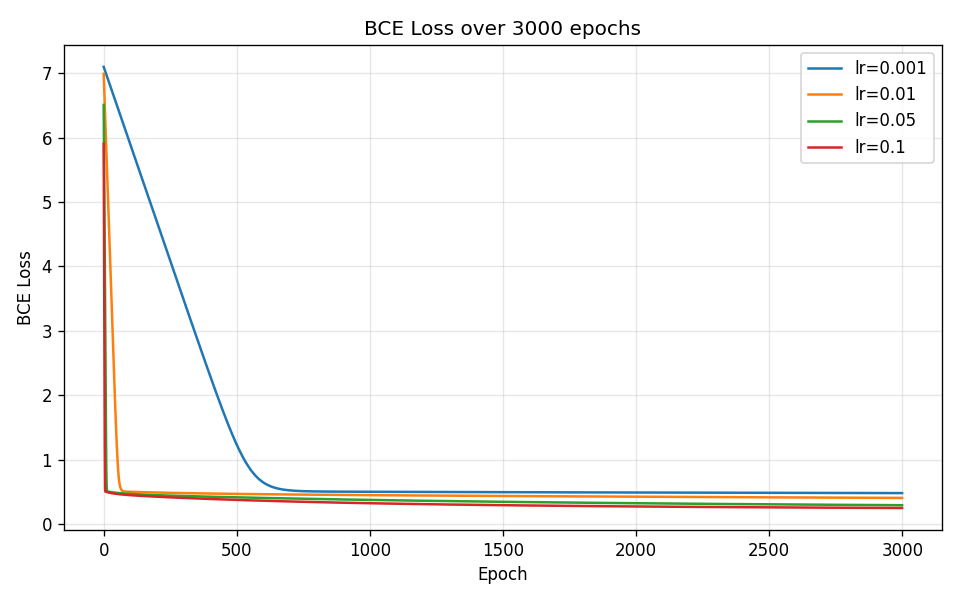
\includegraphics[width=0.85\textwidth]{lor_loss_curves.png}
\caption{BCE loss over 3000 epochs. A larger $r$ leads to a lower final loss within the same number of epochs.}
\end{figure}

\begin{figure}[H]
\centering
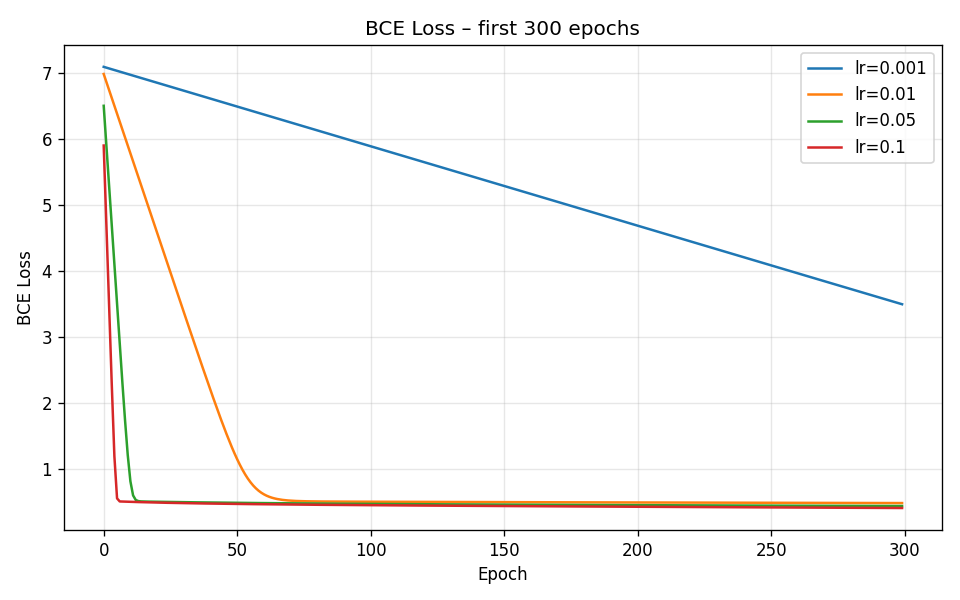
\includegraphics[width=0.85\textwidth]{lor_loss_curves_early.png}
\caption{Loss during the first 300 epochs. The gap in convergence speed is most visible in the early phase.}
\end{figure}

\begin{figure}[H]
\centering
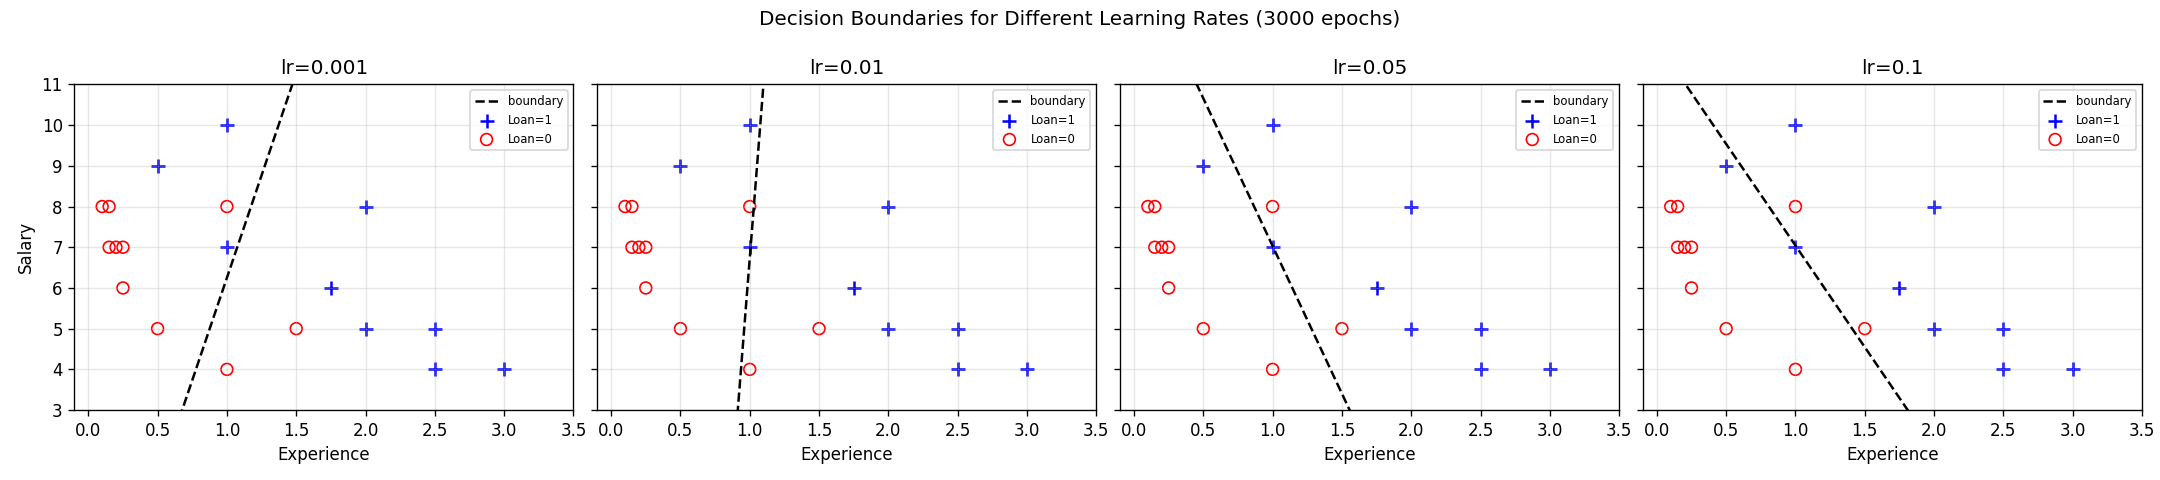
\includegraphics[width=\textwidth]{lor_decision_boundaries.png}
\caption{Decision boundaries (dashed line) after 3000 epochs. ``+'' = Loan, ``o'' = Refuse. A larger $r$ produces a boundary that separates the classes more aggressively.}
\end{figure}

\noindent\textbf{Analysis:}
\begin{itemize}
    \item \textbf{$r = 10^{-3}$:} After 3000 epochs the BCE loss is 0.4824, nearly the same as at epoch 300. The parameters barely move from their initial values, and the decision boundary is almost vertical (dominated by $w_1$).
    \item \textbf{$r = 10^{-2}$:} Loss reaches 0.4074. Convergence is noticeably faster, and $w_0$ has had time to shift meaningfully.
    \item \textbf{$r = 5\times10^{-2}$:} Loss reaches 0.2944. The boundary rotates significantly as $w_2$ (salary) grows positive, showing that the model can better leverage both features.
    \item \textbf{$r = 10^{-1}$:} Loss reaches 0.2509, the best result in this comparison. Larger steps allow faster descent without diverging on this dataset.
    \item \textbf{Too large $r$:} Beyond a safe bound, the weight updates overshoot the minimum and the BCE loss diverges. In practice, $r$ should be validated by monitoring loss stability.
\end{itemize}

\section{Loan Decision Example}

Using the parameters learned with $r = 0.01$ after 3000 epochs ($w_0 = -1.5241$, $w_1 = 1.8056$, $w_2 = -0.0418$), three new employee profiles are evaluated:

\begin{table}[H]
\centering
\caption{Loan decisions for new profiles (threshold $t = 0.5$)}
\begin{tabular}{ccrrc}
\toprule
\textbf{Experience (year)} & \textbf{Salary (M VND)} & $\hat{y}$ & \textbf{Decision} & \textbf{Reasoning} \\
\midrule
2.0 & 7 & 0.8575 & \textbf{LOAN}   & High experience \\
0.1 & 4 & 0.1808 & \textbf{REFUSE} & Low experience \\
1.5 & 8 & 0.7005 & \textbf{LOAN}   & Above-average experience \\
\bottomrule
\end{tabular}
\end{table}

The results confirm that experience is the dominant feature: profiles with experience above $\approx 1$ year are granted loans regardless of salary, while those with very low experience are refused even at moderate salaries.

\section{Conclusion}

I implemented Logistic Regression from scratch using Gradient Descent in pure Python, with no numerical libraries. The algorithm applies the partial derivatives of the Binary Cross-Entropy loss to update $w_0$, $w_1$, and $w_2$ simultaneously. Experiments with four learning rates on the 19-point loan dataset confirm:
\begin{enumerate}
    \item A very small learning rate ($r = 10^{-3}$) results in negligible progress over 3000 epochs.
    \item Increasing the learning rate speeds up convergence, with $r = 10^{-1}$ achieving the lowest final loss.
    \item Experience is the dominant predictor for loan approval in this dataset; the salary weight $w_2$ stays close to zero or even slightly negative, suggesting the two features overlap in information.
    \item Without feature normalisation, gradient descent converges slowly because the gradient scales for $w_1$ and $w_2$ differ according to the feature value ranges.
\end{enumerate}

\end{document}
